% Figure 5.3 (Session 5): the eigenvalues of the correlation matrix as the fillings of cups.
% The image is rendered by figures/blender/s5_3_corr_entropy.py; the coordinates of the labels
% come from figures/blender/out/corr_entropy_anchors.tex. Built by figures/blender/build_figure.sh.
\documentclass[11pt,tikz,border=0pt]{standalone}
\usepackage{amsmath,amssymb,graphicx,braket}
\usepackage{xcolor}
\definecolor{coursedark}{HTML}{1B2A4A}
\definecolor{costamber}{HTML}{B8620A}
\newlength{\figw}\setlength{\figw}{16.19cm}   % the text width of the notes (letter, 2.7 cm margins), so labels print at size

\begin{document}
\begin{tikzpicture}[lbl/.style={font=\small, text=coursedark}]
  \node[anchor=south west, inner sep=0pt] at (0,0)
    {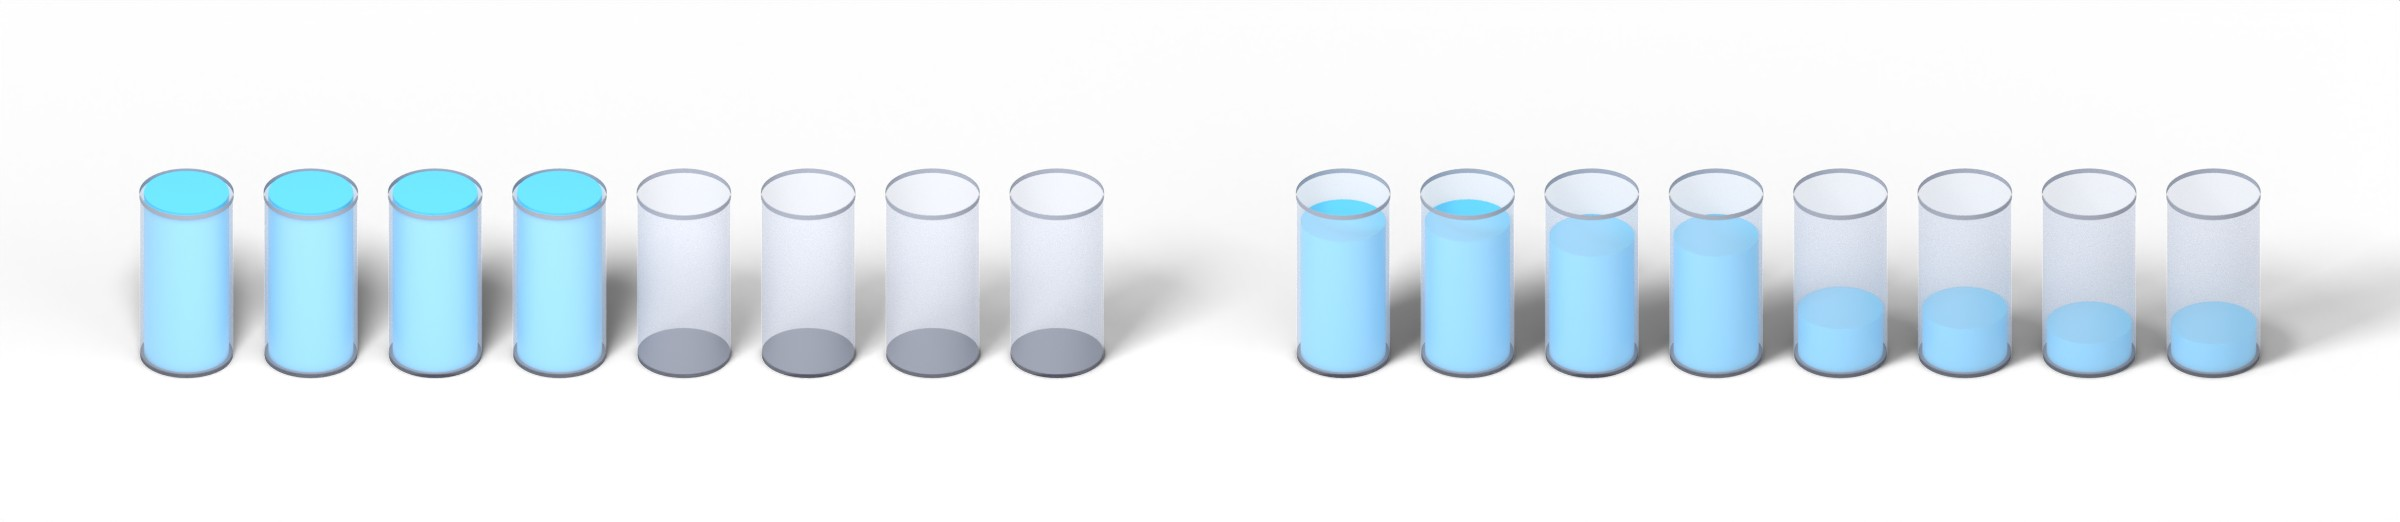
\includegraphics[width=\figw]{../blender/out/corr_entropy.jpg}};
  %% written by figlib.py; x and y in units of the image width
\coordinate (anu0) at (0.0777\figw,0.0561\figw);
\coordinate (anu1) at (0.1295\figw,0.0561\figw);
\coordinate (anu2) at (0.1813\figw,0.0561\figw);
\coordinate (anu3) at (0.2331\figw,0.0561\figw);
\coordinate (anu4) at (0.2849\figw,0.0561\figw);
\coordinate (anu5) at (0.3367\figw,0.0561\figw);
\coordinate (anu6) at (0.3886\figw,0.0561\figw);
\coordinate (anu7) at (0.4404\figw,0.0561\figw);
\coordinate (bnu0) at (0.5596\figw,0.0561\figw);
\coordinate (bnu1) at (0.6114\figw,0.0561\figw);
\coordinate (bnu2) at (0.6633\figw,0.0561\figw);
\coordinate (bnu3) at (0.7151\figw,0.0561\figw);
\coordinate (bnu4) at (0.7669\figw,0.0561\figw);
\coordinate (bnu5) at (0.8187\figw,0.0561\figw);
\coordinate (bnu6) at (0.8705\figw,0.0561\figw);
\coordinate (bnu7) at (0.9223\figw,0.0561\figw);
\coordinate (a) at (0.0241\figw,0.1818\figw);
\coordinate (b) at (0.5060\figw,0.1818\figw);
\coordinate (Sa) at (0.2771\figw,0.1609\figw);
\coordinate (Sb) at (0.7590\figw,0.1609\figw);

  \node[lbl, font=\normalsize, anchor=west] at (a) {(a)};
  \node[lbl, font=\normalsize, anchor=west] at (b) {(b)};
  \node[lbl, anchor=south] at (Sa) {$U=0$:\quad $\nu_k\in\{0,1\}$,\quad $S_{\mathrm{corr}}=0$};
  \node[lbl, anchor=south] at (Sb) {$U=6t$:\quad $0<\nu_k<1$,\quad $S_{\mathrm{corr}}=4.22$};
  \foreach \k/\v in {0/1,1/1,2/1,3/1,4/0,5/0,6/0,7/0} \node[lbl, anchor=north] at (anu\k) {$\v$};
  \foreach \k/\v in {0/0.82,1/0.82,2/0.73,3/0.73,4/0.27,5/0.27,6/0.18,7/0.18} \node[lbl, anchor=north] at (bnu\k) {$\v$};
\end{tikzpicture}
\end{document}
